\section{MIPS} \label{sec_mips}
Ao contrário dos programas nas linguagens de alto nível, os operandos das instruções aritméticas são restritos, precisam ser de um grupo limitado de locais especiais, embutidos diretamente no hardware, chamados \textit{registradores}. Uma diferença importante entre as variáveis de uma linguagem de programação e os registradores é o número limitado de registradores, o MIPS possui 32 registradores com tamanho de 32 bits cada \cite{patterson1}. O nome dos registradores e as indicaões de uso podem ser conferidos na Tabela~{\ref{tab:tabela-mips-001}}.

\begin{table}[b]
\caption {Registradores do MIPS}
\begin{center}
\begin{tabularx}{8.4cm}{llX} 
\textbf{Nome} & \textbf{Número} & \textbf{Uso} \\ \hline
\$zero & 0 & O valor constante 0 \\ \hline
\$at & 1 & Temporário do montador\\ \hline
\$v0-\$v1 & 2-3 & Valores para resultados de função e avaliação de expressão\\ \hline
\$a0-\$a3 & 4-7 & Argumentos \\ \hline
\$t0-\$t7 & 8-15 & Temporários \\ \hline
\$s0-\$s7 & 16-23 & Temporários salvos \\ \hline
\$t8-\$t9 & 24-25 & Temporários \\ \hline
\$k0-\$k1 & 26-27 & Reservados para kernel do SO \\ \hline
\$gp & 28 & Ponteiro global \\ \hline
\$sp & 29 & Stack Pointer \\ \hline
\$fp & 30 & Frame Pointer \\ \hline
\$ra & 31 & Endereço de retorno \\ \hline
\end{tabularx}
\end{center}
\label{tab:tabela-mips-001}
\end{table}

\subsection{Formato das Instruções}

Existem três tipos de instruções no MIPS. As instruções do tipo Registrador Tipo-R (\textit{R-Type}) realizam operações aritméticas e lógicas com dados buscados do banco de registradores, salvando no mesmo a resposta da operação. Esse tipo de instrução possui 6 campos, o código do campo \textit{Opcode}, de 6 bits, junto com o campo \textit{Funct}, também de 6 bits, informam qual operação será realizada. Os campos \textit{Rs} e \textit{Rt} indicam os registradores de origem e o campo \textit{Rd} indica o registrador de destino da operação, o campo \textit{Shamt} informa quantos bits devem ser deslocados, para esquerda ou para a direita, todos possuem 5 bits. Instruções do Tipo-I (\textit{I-Type}) são utilizadas de várias formas - operações aritméticas e lógicas, desvios condicionais, leitura e escrita na memória de dados \cite{cruz1} - possuem 4 campos, diferindo do Tipo-R por apresentar o campo \textit{IMM} de 16 bits e somente dois registradores, \textit{Rs} e \textit{Rt}, além do \textit{Opcode} como pode ser visto na Figura~{\ref{fig:figura-mips-001}}.

\begin{figure}[h]
    \centering
    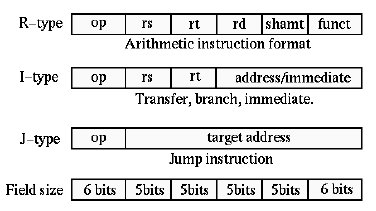
\includegraphics[width=0.48 \textwidth]{figuras/MIPS-Instruction-Type_W840.jpg}
    \caption{Tipos de Instruões do MIPS \cite{misc1}}
    \label{fig:figura-mips-001}
\end{figure}

Por último temos as instruções do \textit{Jump}, \textit{J-Type}, composta pelo \textit{Opcode} e pelo campo endereço \textit{addr} de 26 bits, responsáveis por desvios, retornos e saltos de instruções.

\subsection{Instruções Básicas}
Para melhor ilustrar as instruções 
